\subsection{Online advisors on all three tasks}
\label{sec:supp:online120}

We repeated the selective online-advising comparison on DoorKey-$8\times8$,
MultiRoom-N6 and KeyCorridor-S3R3 with at most 120 GPT-5-mini requests per
training run. All other settings follow the earlier study: a teacher with
full-map access, recurrent PPO or Count-PPO with local $7\times7$ symbolic
observations, 9,999,360 transitions, an imitation coefficient decaying from
1.0 to 0.01, and five paired training seeds per task. Entropy-based queries
request advice when the student's normalized policy entropy is high;
probability correction delivers the teacher's action as a target only when
the student assigns it probability below 0.2; random timing draws query
slots uniformly within the advice period. Delivered labels can be fewer
than requests. No-advice controls, the DoorKey and MultiRoom Count-PPO
random-timing runs and both KeyCorridor random-timing arms are completed
runs with identical settings and seeds. The remaining runs used a different
cluster: they share training seeds and settings with their controls but
not the initial network weights.

\begin{table}[htbp]\centering\small
\setlength{\tabcolsep}{4pt}
\caption{Online advisors with 120 requests per run: mean greedy AUC, with
mean final greedy success (\%) in parentheses. Five paired seeds, 10M
transitions.}
\label{tab:supp:online120}
\begin{tabular}{@{}llrrrr@{}}
\toprule
Task & Student & No advice & Entropy & Mistake corr. & Random \\
\midrule
DoorKey     & PPO       & .003 (3.6) & .000 (0) & .000 (0) & .000 (0) \\
            & Count-PPO & .719 (100) & .936 (100) & .864 (100) & .787 (100) \\
MultiRoom   & PPO       & .000 (0) & .000 (0) & .000 (0) & .000 (0) \\
            & Count-PPO & .348 (40) & .927 (100) & .948 (100) & .956 (99.6) \\
KeyCorridor & PPO       & .000 (0) & .000 (0) & .000 (0) & .000 (0) \\
            & Count-PPO & .936 (100) & .966 (100) & .980 (100) & .775 (80) \\
\bottomrule
\end{tabular}
\end{table}

Paired Count-PPO AUC gains over no advice (entropy, mistake correction,
random) are $+.216$, $+.145$ and $+.068$ on DoorKey; $+.579$, $+.600$ and
$+.608$ on MultiRoom; and $+.030$, $+.045$ and $-.161$ on KeyCorridor. No
gain is significant after Holm correction over the three advisors (smallest
adjusted $p=.138$). The earlier 480-request cohorts agree: with entropy
queries or mistake correction, plain PPO has 0\% final success on DoorKey
and MultiRoom, and random timing reaches 19.2\% on DoorKey from one seed.
The 8,395 requests cost \$32.25. Failed requests are 0.1\% on DoorKey and
about 8\% on MultiRoom and KeyCorridor, mostly replies cut off at the
output limit; a failed request delivers no label.

\begin{figure}[htbp]\centering
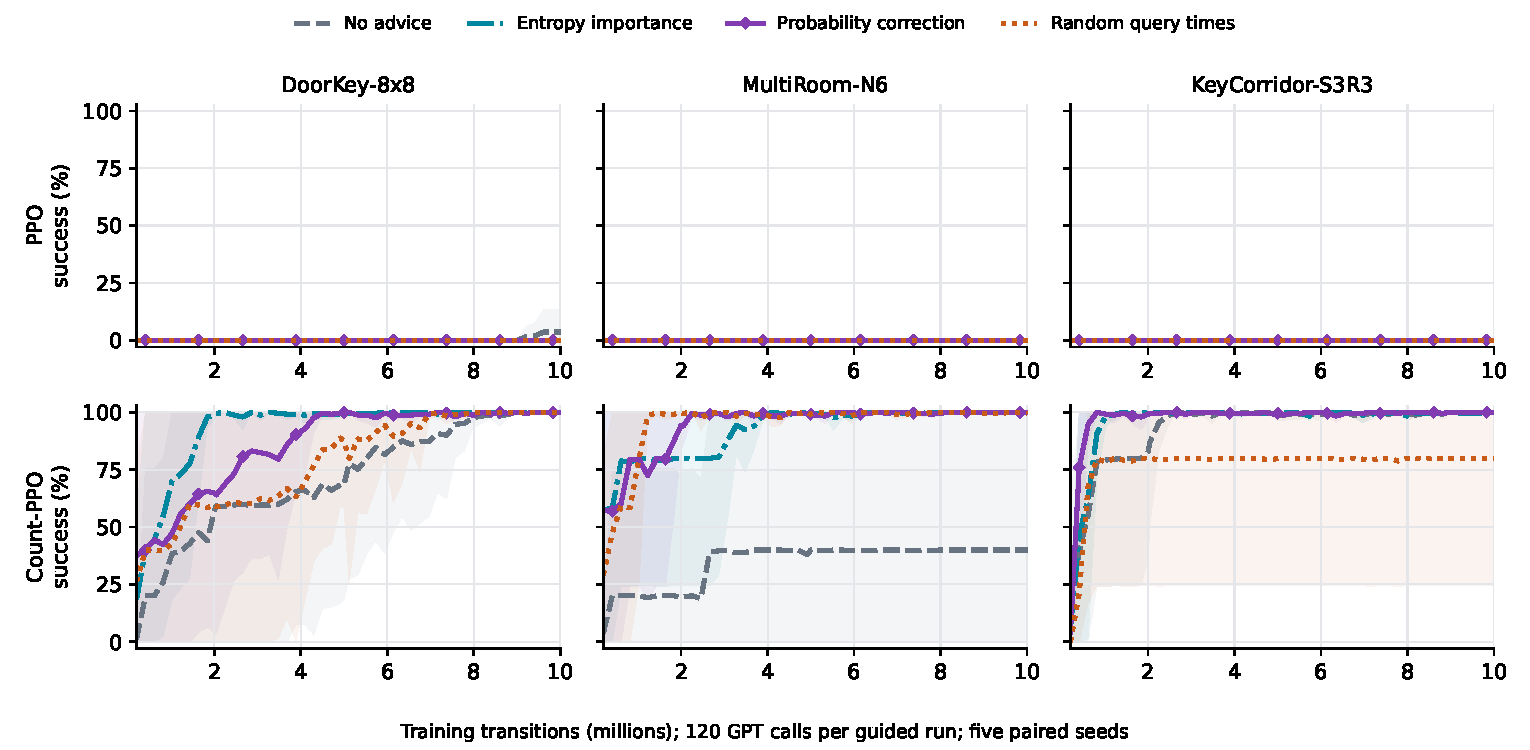
\includegraphics[width=\linewidth]{figures/online_advisors_120calls.pdf}
\caption{Online GPT-5-mini advisors with 120 requests per run on the three
source tasks. Teacher-free greedy success; lines are means over five
paired seeds and bands pointwise 95\% $t$-intervals clipped to
$[0,100]\%$. Plain PPO remains at 0\% with every advisor.}
\label{fig:supp:online120}
\end{figure}
